%=========PROBLEM 5============================================
\section*{Problem 5}

All computers treat numbers as approximation to the nearest bit representation of that number. It will greatly differ by the amount of bits used and the type of number. Numbers that are type \textit{int} are always exact but that is not the case for example to numbers of type \textit{float}. In addition, the values between different data types but same operation will differ notably. This is an unstability. This exercise asks to show the unstability of the "Golden Mean Ratio" when using the following equation, 

\begin{equation}
    \phi^{n+1}=\phi^{n-1}-\phi^{n}
\end{equation}

Knowing that $\phi^0=1$ and $\phi^1=\frac{\sqrt{5}-1}{2}$, the previous formula becomes a subtraction of known values. An easier way to see it is that equation becomes "the future value of $\phi$ is equal to the past value - the present value". In this way, if we are on the first iteration, the present value is $\phi^n$ which is a known value and $\phi^{n=1}$ aka the future value is calculated. 

The values of $\phi$ can be seen in Figure \ref{fig:phi}.

\begin{figure}
    \centering
    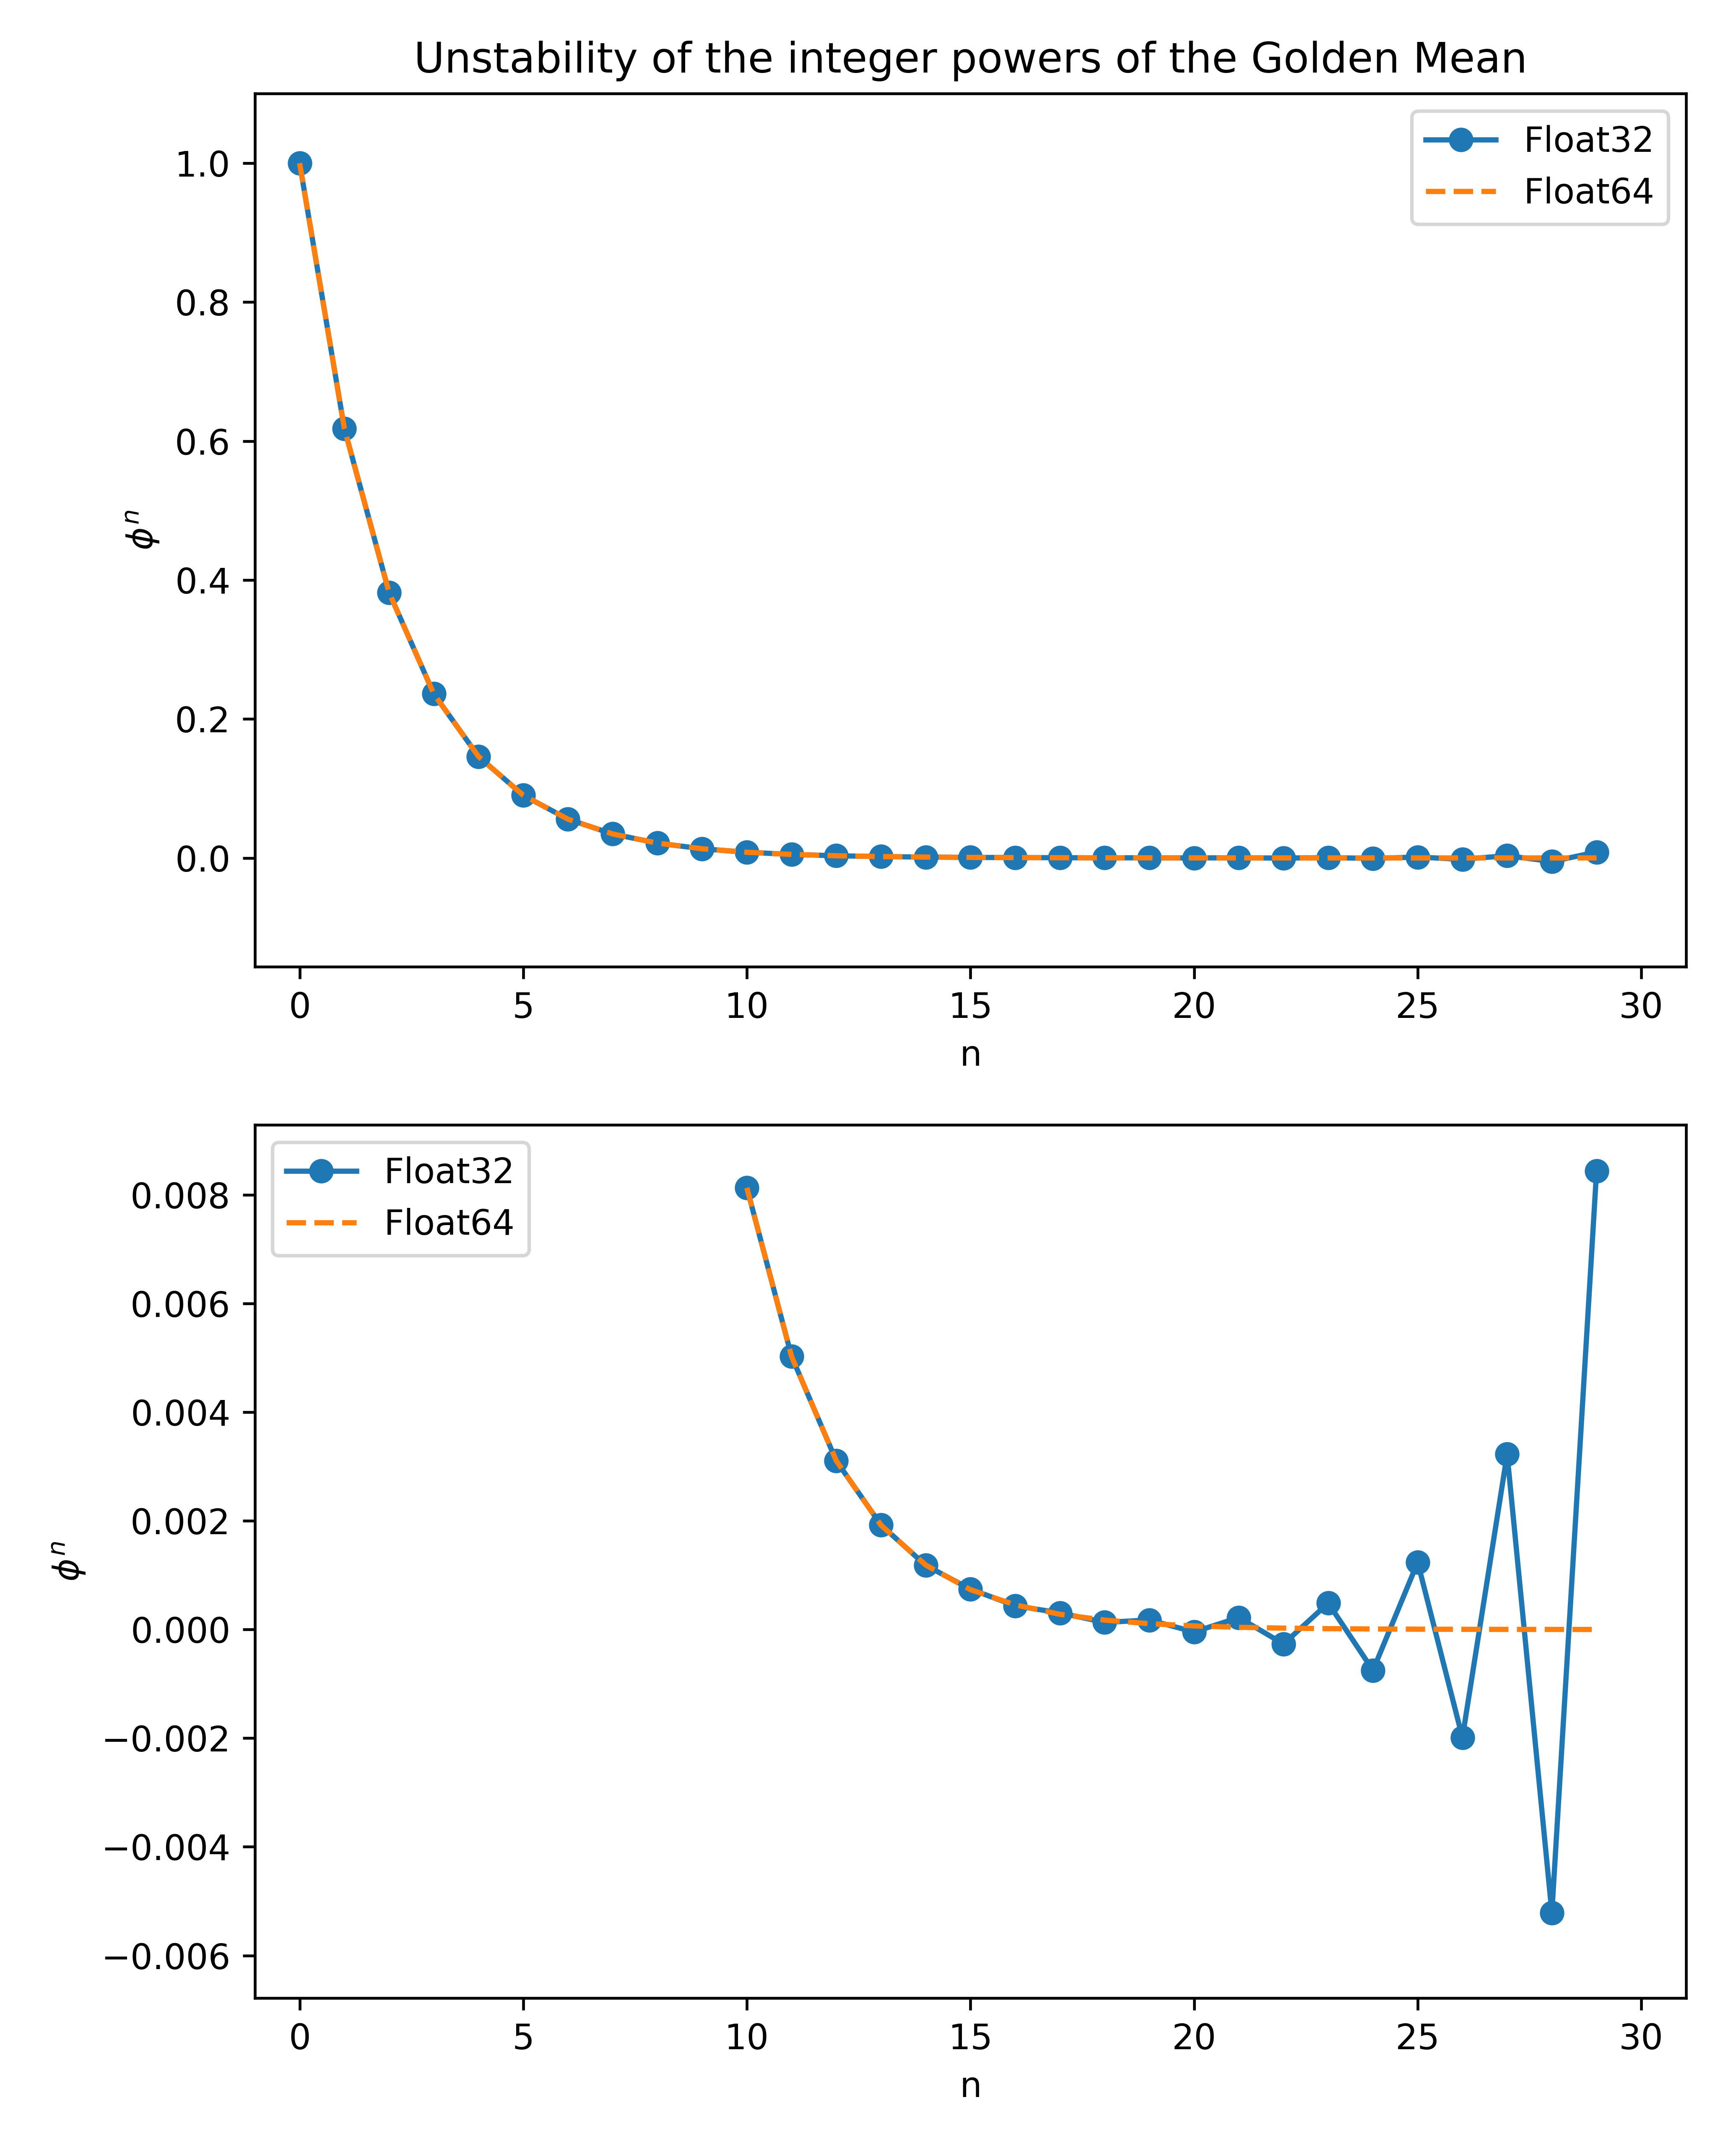
\includegraphics{figures/hw01prob1-5fig1.png}
    \caption{Top: Shows the values of $\phi$ using the Golden Mean Recursion. Bottom: Shows a zoom so that the differences are more clearly seen.}
    \label{fig:phi}
\end{figure}